% !Mode:: "TeX:UTF-8"
\documentclass[12pt,a4paper]{article}

%%%%%%%%------------------------------------------------------------------------
%%%% 日常所用宏包

%% 控制页边距
% 如果是beamer文档类, 则不用geometry
\makeatletter
\@ifclassloaded{beamer}{}{\usepackage[top=2.5cm, bottom=2.5cm, left=2.5cm, right=2.5cm]{geometry}}
\makeatother

%% 控制项目列表
\usepackage{enumerate}

%% 多栏显示
\usepackage{multicol}

%% 算法环境
\usepackage{algorithm}  
\usepackage{algorithmic} 
\usepackage{float} 

%% 网址引用
\usepackage{url}

%% 控制矩阵行距
\renewcommand\arraystretch{1.4}

%% hyperref宏包,生成可定位点击的超链接,并且会生成pdf书签
\makeatletter
\@ifclassloaded{beamer}{
\usepackage{hyperref}
\usepackage{ragged2e} % 对齐
}{
\usepackage[%
    pdfstartview=FitH,%
    CJKbookmarks=true,%
    bookmarks=true,%
    bookmarksnumbered=true,%
    bookmarksopen=true,%
    colorlinks=true,%
    citecolor=blue,%
    linkcolor=blue,%
    anchorcolor=green,%
    urlcolor=blue%
]{hyperref}
}
\makeatother



\makeatletter % 如果是 beamer 不需要下面两个包
\@ifclassloaded{beamer}{
\mode<presentation>
{
} 
}{
%% 控制标题
\usepackage{titlesec}
%% 控制目录
\usepackage{titletoc}
}
\makeatother

%% 控制表格样式
\usepackage{booktabs}

%% 控制字体大小
\usepackage{type1cm}

%% 首行缩进,用\noindent取消某段缩进
\usepackage{indentfirst}

%%边框
\usepackage{listings}

%% 支持彩色文本、底色、文本框等
\usepackage{color,xcolor}

%% AMS LaTeX宏包: http://zzg34b.w3.c361.com/package/maths.htm#amssymb
\usepackage{amsmath,amssymb}
%% 多个图形并排
\usepackage{subfig}
%%%% 基本插图方法
%% 图形宏包
\usepackage{graphicx}
\newcommand{\red}[1]{\textcolor{red}{#1}}
\newcommand{\blue}[1]{\structure{#1}}
\newcommand{\brown}[1]{\textcolor{brown}{#1}}
\newcommand{\green}[1]{\textcolor{green}{#1}}


%%%% 基本插图方法结束

%%%% pgf/tikz绘图宏包设置
\usepackage{pgf,tikz}
\usetikzlibrary{shapes,automata,snakes,backgrounds,arrows}
\usetikzlibrary{mindmap}
%% 可以直接在latex文档中使用graphviz/dot语言,
%% 也可以用dot2tex工具将dot文件转换成tex文件再include进来
%% \usepackage[shell,pgf,outputdir={docgraphs/}]{dot2texi}
%%%% pgf/tikz设置结束


\makeatletter % 如果是 beamer 不需要下面两个包
\@ifclassloaded{beamer}{

}{
%%%% fancyhdr设置页眉页脚
%% 页眉页脚宏包
\usepackage{fancyhdr}
%% 页眉页脚风格
\pagestyle{plain}
}

%% 有时会出现\headheight too small的warning
\setlength{\headheight}{15pt}

%% 清空当前页眉页脚的默认设置
%\fancyhf{}
%%%% fancyhdr设置结束


\makeatletter % 对 beamer 要重新设置
\@ifclassloaded{beamer}{

}{
%%%% 设置listings宏包用来粘贴源代码
%% 方便粘贴源代码,部分代码高亮功能
\usepackage{listings}

%% 设置listings宏包的一些全局样式
%% 参考http://hi.baidu.com/shawpinlee/blog/item/9ec431cbae28e41cbe09e6e4.html
\lstset{
showstringspaces=false,              %% 设定是否显示代码之间的空格符号
numbers=left,                        %% 在左边显示行号
numberstyle=\tiny,                   %% 设定行号字体的大小
basicstyle=\footnotesize,                    %% 设定字体大小\tiny, \small, \Large等等
keywordstyle=\color{blue!70}, commentstyle=\color{red!50!green!50!blue!50},
                                     %% 关键字高亮
frame=shadowbox,                     %% 给代码加框
rulesepcolor=\color{red!20!green!20!blue!20},
escapechar=`,                        %% 中文逃逸字符,用于中英混排
xleftmargin=2em,xrightmargin=2em, aboveskip=1em,
breaklines,                          %% 这条命令可以让LaTeX自动将长的代码行换行排版
extendedchars=false                  %% 这一条命令可以解决代码跨页时,章节标题,页眉等汉字不显示的问题
}}
\makeatother
%%%% listings宏包设置结束


%%%% 附录设置
\makeatletter % 对 beamer 要重新设置
\@ifclassloaded{beamer}{

}{
\usepackage[title,titletoc,header]{appendix}
}
\makeatother
%%%% 附录设置结束


%%%% 日常宏包设置结束
%%%%%%%%------------------------------------------------------------------------


%%%%%%%%------------------------------------------------------------------------
%%%% 英文字体设置结束
%% 这里可以加入自己的英文字体设置
%%%%%%%%------------------------------------------------------------------------

%%%%%%%%------------------------------------------------------------------------
%%%% 设置常用字体字号,与MS Word相对应

%% 一号, 1.4倍行距
\newcommand{\yihao}{\fontsize{26pt}{36pt}\selectfont}
%% 二号, 1.25倍行距
\newcommand{\erhao}{\fontsize{22pt}{28pt}\selectfont}
%% 小二, 单倍行距
\newcommand{\xiaoer}{\fontsize{18pt}{18pt}\selectfont}
%% 三号, 1.5倍行距
\newcommand{\sanhao}{\fontsize{16pt}{24pt}\selectfont}
%% 小三, 1.5倍行距
\newcommand{\xiaosan}{\fontsize{15pt}{22pt}\selectfont}
%% 四号, 1.5倍行距
\newcommand{\sihao}{\fontsize{14pt}{21pt}\selectfont}
%% 半四, 1.5倍行距
\newcommand{\bansi}{\fontsize{13pt}{19.5pt}\selectfont}
%% 小四, 1.5倍行距
\newcommand{\xiaosi}{\fontsize{12pt}{18pt}\selectfont}
%% 大五, 单倍行距
\newcommand{\dawu}{\fontsize{11pt}{11pt}\selectfont}
%% 五号, 单倍行距
\newcommand{\wuhao}{\fontsize{10.5pt}{10.5pt}\selectfont}
%%%%%%%%------------------------------------------------------------------------


%% 设定段间距
\setlength{\parskip}{0.5\baselineskip}

%% 设定行距
\linespread{1}


%% 设定正文字体大小
% \renewcommand{\normalsize}{\sihao}

%制作水印
\RequirePackage{draftcopy}
\draftcopyName{XTUMESH}{100}
\draftcopySetGrey{0.90}
\draftcopyPageTransform{40 rotate}
\draftcopyPageX{350}
\draftcopyPageY{80}

%%%% 个性设置结束
%%%%%%%%------------------------------------------------------------------------


%%%%%%%%------------------------------------------------------------------------
%%%% bibtex设置

%% 设定参考文献显示风格
% 下面是几种常见的样式
% * plain: 按字母的顺序排列,比较次序为作者、年度和标题
% * unsrt: 样式同plain,只是按照引用的先后排序
% * alpha: 用作者名首字母+年份后两位作标号,以字母顺序排序
% * abbrv: 类似plain,将月份全拼改为缩写,更显紧凑
% * apalike: 美国心理学学会期刊样式, 引用样式 [Tailper and Zang, 2006]

\makeatletter
\@ifclassloaded{beamer}{
\bibliographystyle{apalike}
}{
\bibliographystyle{unsrt}
}
\makeatother


%%%% bibtex设置结束
%%%%%%%%------------------------------------------------------------------------

%%%%%%%%------------------------------------------------------------------------
%%%% xeCJK相关宏包

\usepackage{xltxtra,fontspec,xunicode}
\usepackage[slantfont, boldfont]{xeCJK} 

\setlength{\parindent}{2em}%中文缩进两个汉字位

%% 针对中文进行断行
\XeTeXlinebreaklocale "zh"             

%% 给予TeX断行一定自由度
\XeTeXlinebreakskip = 0pt plus 1pt minus 0.1pt

%%%% xeCJK设置结束                                       
%%%%%%%%------------------------------------------------------------------------
\usepackage{ listings} 
\usepackage{ xcolor}
%%%%%%%%------------------------------------------------------------------------
%%%% xeCJK字体设置

%% 设置中文标点样式,支持quanjiao、banjiao、kaiming等多种方式
\punctstyle{kaiming}                                        
\usepackage{framed}%%边框                                                
%% 设置缺省中文字体
%\setCJKmainfont[BoldFont={Adobe Heiti Std}, ItalicFont={Adobe Kaiti Std}]{Adobe Song Std}   
\setCJKmainfont{SimSun}
%% 设置中文无衬线字体
%\setCJKsansfont[BoldFont={Adobe Heiti Std}]{Adobe Kaiti Std}  
%% 设置等宽字体
%\setCJKmonofont{Adobe Heiti Std}                            

%% 英文衬线字体
\setmainfont{DejaVu Serif}                                  
%% 英文等宽字体
\setmonofont{DejaVu Sans Mono}                              
%% 英文无衬线字体
\setsansfont{DejaVu Sans}                                   

%% 定义新字体
\setCJKfamilyfont{song}{Adobe Song Std}                     
\setCJKfamilyfont{kai}{Adobe Kaiti Std}
\setCJKfamilyfont{hei}{Adobe Heiti Std}
\setCJKfamilyfont{fangsong}{Adobe Fangsong Std}
\setCJKfamilyfont{lisu}{LiSu}
\setCJKfamilyfont{youyuan}{YouYuan}

%% 自定义宋体
\newcommand{\song}{\CJKfamily{song}}                       
%% 自定义楷体
\newcommand{\kai}{\CJKfamily{kai}}                         
%% 自定义黑体
\newcommand{\hei}{\CJKfamily{hei}}                         
%% 自定义仿宋体
\newcommand{\fangsong}{\CJKfamily{fangsong}}               
%% 自定义隶书
\newcommand{\lisu}{\CJKfamily{lisu}}                       
%% 自定义幼圆
\newcommand{\youyuan}{\CJKfamily{youyuan}}                 

%%%% xeCJK字体设置结束
%%%%%%%%------------------------------------------------------------------------

%%%%%%%%------------------------------------------------------------------------
%%%% 一些关于中文文档的重定义
\newcommand{\chntoday}{\number\year\,年\,\number\month\,月\,\number\day\,日}
%% 数学公式定理的重定义

%% 中文破折号,据说来自清华模板
\newcommand{\pozhehao}{\kern0.3ex\rule[0.8ex]{2em}{0.1ex}\kern0.3ex}

\newtheorem{example}{例}                                   
\newtheorem{theorem}{定理}[section]                         
\newtheorem{definition}{定义}
\newtheorem{axiom}{公理}
\newtheorem{property}{性质}
\newtheorem{proposition}{命题}
\newtheorem{lemma}{引理}
\newtheorem{corollary}{推论}
\newtheorem{remark}{注解}
\newtheorem{condition}{条件}
\newtheorem{conclusion}{结论}
\newtheorem{assumption}{假设}

\makeatletter %
\@ifclassloaded{beamer}{

}{
%% 章节等名称重定义
\renewcommand{\contentsname}{目录}     
\renewcommand{\indexname}{索引}
\renewcommand{\listfigurename}{插图目录}
\renewcommand{\listtablename}{表格目录}
\renewcommand{\appendixname}{附录}
\renewcommand{\appendixpagename}{附录}
\renewcommand{\appendixtocname}{附录}
%% 设置chapter、section与subsection的格式
\titleformat{\chapter}{\centering\huge}{第\thechapter{}章}{1em}{\textbf}
\titleformat{\section}{\centering\sihao}{\thesection}{1em}{\textbf}
\titleformat{\subsection}{\xiaosi}{\thesubsection}{1em}{\textbf}
\titleformat{\subsubsection}{\xiaosi}{\thesubsubsection}{1em}{\textbf}

\@ifclassloaded{book}{

}{
\renewcommand{\abstractname}{摘要}
}
}
\makeatother

\renewcommand{\figurename}{图}
\renewcommand{\tablename}{表}

\makeatletter
\@ifclassloaded{book}{
\renewcommand{\bibname}{参考文献}
}{
\renewcommand{\refname}{参考文献} 
}
\makeatother

\floatname{algorithm}{算法}
\renewcommand{\algorithmicrequire}{\textbf{输入:}}
\renewcommand{\algorithmicensure}{\textbf{输出:}}

%%%% 中文重定义结束
%%%%%%%%------------------------------------------------------------------------


\title{矩阵计算}
\author{潘建瑜}

\begin{document}
\section{线性方程组直接解法}

{\bfseries 线性方程组的求解方法}

• 直接法: $LU$ 分解, $Cholesky$ 分解, ...

• 迭代法: 古典迭代法, $Krylov$ 子空间迭代法

本章介绍直接法, 即 Gauss 消去法 或 PLU 分解

直接法优点: 稳定可靠 → 在工程界很受欢迎

直接法缺点: 运算量大 $O(n^3)$ → 不适合大规模稀疏线性方程组(针对特殊结构矩阵的快速方法除外)

\subsection{Gauss 消去法和 LU 分解}

4.1.1 $LU$ 分解

4.1.2 $LU$ 分解的实现

4.1.3 $IKJ$ 型 $LU$ 分解

4.1.4 待定系数法计算 $LU$ 分解

4.1.5 三角方程求解

4.1.6 选主元 $LU$ 分解

4.1.7 矩阵求逆

\subsubsection{LU 分解}
考虑线性方程组
\begin{equation}
A x=b
\end{equation}
其中 $A ∈ \mathbb{R}^{n×n}$ 非奇异, $b ∈ \mathbb{R}^n$ 为给定的右端项.

\begin{framed}
	Gauss 消去法本质上就是对系数矩阵 A 进行 LU 分解:
	\begin{equation}
	A=L U
	\end{equation}
	其中 L 是单位下三角矩阵, U 为非奇异上三角矩阵.
\end{framed}

分解()就称为$LU$分解

\begin{equation}
A x=b \Longleftrightarrow\left\{\begin{array}{l}{L y=b} \\ {U x=y}\end{array} | \Longrightarrow \text{ 只需求解两个三角方程组} \right.
\end{equation}

\begin{table}  
	%\caption{设置表格总长}  
	\begin{tabular*}{16cm}{ll}  
		\hline  
		算法4.1: & Gauss 消去法 \\  
		\hline  
		1:   &将 $A$ 进行 $LU$ 分解:\\  
		2:   &$A = LU$, 其中 $L$ 为单位下三角矩阵, $U$ 为非奇异上三角矩阵;\\
		3:   &向前回代: 求解 $Ly = b$, 即得$ y = L^{-1}b$\\
		4:   &向后回代: 求解 $Ux = y$, 即得 $x = U^{-1}y = (LU)^{-1}b = A^{-1}b$.\\  
		\hline  
	\end{tabular*}  
\end{table} 

 \begin{framed}
 	$†$ 需要指出的是: $A$ 非奇异, 则解存在唯一, 但并不一定存在 $LU$ 分解!
 \end{framed}

\begin{framed}
	\begin{theorem}(LU 分解的存在性和唯一性)
	设 $A ∈ \mathbb{R}^{n×n}$. 则存在唯一的单位下
	三角矩阵 $L$ 和非奇异上三角矩阵 $U$, 使得 $A = LU$ 的充要条件是 $A$ 的
	所有顺序主子矩阵 $A_k = A(1:k, 1:k)$ 都非奇异, $k = 1, 2, . . . , n.$	
	\end{theorem}
\end{framed}

\newpage
\subsubsection{LU 分解的实现 — 矩阵初等变换}
给定一个矩阵
\begin{equation*}
A=\left[\begin{array}{cccc}{a_{11}} & {a_{12}} & {\cdots} & {a_{1 n}} \\ {a_{21}} & {a_{22}} & {\cdots} & {a_{2 n}} \\ {\vdots} & {} & {\ddots} & {} \\ {a_{n 1}} & {a_{n 2}} & {\cdots} & {a_{n n}}\end{array}\right] \in \mathbb{R}^{n \times n}
\end{equation*}

• 第一步: 假定 $a_{11} \neq  0$, 构造矩阵

\centering {$L_{1}=\left[\begin{array}{ccccc}{1} & {0} & {0} & {\cdots} & {0} \\ {l_{21}} & {1} & {0} & {\cdots} & {0} \\ {l_{31}} & {0} & {1} & {\cdots} & {0} \\ {\vdots} & {} & {} & {\ddots} \\ {l_{n 1}} & {0} & {0} & {\cdots} & {1}\end{array}\right]$ $\text{,其中}$ $l_{i 1}=\frac{a_{i 1}}{a_{11}}, i=2,3, \dots, n $}
\\
易知 $L_1$ 的逆为
$$
L_{1}^{-1}=\left[\begin{array}{ccccc}{1} & {0} & {0} & {\cdots} & {0} \\ {-l_{21}} & {1} & {0} & {\cdots} & {0} \\ {-l_{31}} & {0} & {1} & {\cdots} & {0} \\ {\vdots} & {} & {\ddots} & {} \\ {-l_{n 1}} & {0} & {0} & {\cdots} & {1}\end{array}\right]
$$
\\
用 $L^{−1}_1 $左乘 $A$, 并将所得到的矩阵记为 $A(1)$
, 则
$$
A^{(1)}=L_{1}^{-1} A\left[\begin{array}{cccc}{a_{11}} & {a_{12}} & {\cdots} & {a_{1 n}} \\ {0} & {a_{22}^{(1)}} & {\cdots} & {a_{2 n}^{(1)}} \\ {\vdots} & {\vdots} & {\ddots} & {} \\ {0} & {a_{n 2}^{(1)}} & {\cdots} & {a_{n n}^{(1)}}\end{array}\right]
$$
\\
即左乘 $L^{−1}_1 $后, $A$ 的第一列中除第一个元素外其它都变为$ 0$.
\\
• 第二步: 将上面的操作作用在 $A^{(1)}$ 的子矩阵 $A^{(1)}(2 : n, 2 : n)$ 上, 将
其第一列除第一个元素外都变为 $0:$ 假定$ a^{(1)}_{22} \neq 0$, 构造矩阵

\centering {$L_{2}=\left[\begin{array}{ccccc}{1} & {0} & {0} & {\cdots} & {0} \\ {0} & {1} & {0} & {\cdots} & {0} \\ {0} & {l_{32}} & {1} & {\cdots} & {0} \\ {\vdots} & {\vdots} & {\ddots} & {\ddots} \\ {0} & {l_{n 2}} & {0} & {\cdots} & {1}\end{array}\right]$ $\text{,其中}$ $l_{i 2}=\frac{a_{i 2}^{(1)}}{a_{22}^{(1)}}, i=3,4, \ldots, n$}

用$L_{2}^{-1}$左乘$A^{(1)}$
, 并将所得到的矩阵记为$A^{(2)}$
, 则
$$
A^{(2)}=L_{2}^{-1} A=L_{2}^{-1} L_{1}^{-1}A=\left[\begin{array}{ccccc}{a_{11}} & {a_{12}} & {a_{13}} & {\dots} &{a_{1 n}} \\ {0} & {a_{22}^{(1)}} & {a_{23}^{(1)}} & {\dots} & {a_{2 n}^{(1)}} \\ {0} & {0} & {a_{33}^{(2)}} & {\dots} & {a_{3 n}^{(2)}} \\ {\vdots} & {\vdots} & {\vdots} & {\ddots} &{ } \\ {0} & {0} & {a_{n 3}^{(2)}} & {\cdots} & {a_{n n}^{(2)}}\end{array}\right]
$$

依此类推, 假定$a_{k k}^{(k-1)} \neq 0(k=3,4, \dots, n-1)$, 则我们可以构造一系
列的矩阵$ L_3, L_4, . . . , L_{n−1}$, 使得
$$
L_{n-1}^{-1} \cdots L_{2}^{-1} L_{1}^{-1} A=\left[\begin{array}{ccccc}{a_{11}} & {a_{12}} & {a_{13}} & {\dots} & {a_{1 n}} \\ {0} & {a_{22}^{(1)}} & {a_{23}^{(1)}} & {\dots} & {a_{2 n}^{(1)}} \\ {0} & {0} & {a_{33}^{(2)}} & {\cdots} & {a_{3 n}^{(2)}} \\ {\vdots} & {\vdots} & {\vdots} & {\ddots} \\ {0} & {0} & {0} & {\cdots} & {a_{n n}^{(n-1)}}\end{array}\right] \triangleq U \rightarrow \text{上三角}
$$

于是可得 $A = LU$ 其中
$$
L=L_{1} L_{2} \cdots L_{n-1}=\left[\begin{array}{ccccc}{1} & {0} & {0} & {\cdots} &{0}\\ {l_{21}} & {1} & {0} & {\cdots} &{0}\\ {l_{31}} & {l_{32}} & {1} & {\cdots} &{0}\\ {\vdots} & {\vdots} & { }& {\ddots} & { }\\ {l_{n 1}} & {l_{n 2}} & {l_{n 3}} & {\cdots} &{1}\end{array}\right]
$$

\begin{table}  
	%\caption{设置表格总长}  
	\begin{tabular*}{16cm}{ll}  
		\hline  
		算法4.2: &LU 分解 \\  
		\hline  
		1:   &for k = 1 to n − 1 do\\  
		2:   &\qquad for i = k + 1 to n do\\
		3:   &\qquad \qquad $l_{ik} = a_{ik}/a_{kk}$ \% 计算 L 的第 k 列\\
		4:   &\qquad end for\\
		5:   &\qquad for j = k to n do\\
		6:   &\qquad \qquad $u_{kj} = a_{kj}$ \% 计算 U 的第 k 行\\
		7:   &\qquad end for\\
		8:   &\qquad end for i = k + 1 to n do\\
		9:   & \qquad \qquad for j = k + 1 to n do\\
		10:   &\qquad \qquad \qquad $a_{ij}= a_{ij} − l_{ik}u_{kj}$ \% 更新 A(k + 1 : n, k + 1 : n)\\
		11:   &\qquad \qquad end for\\
		12:   &\qquad end for\\
		13:   &end for\\
		\hline  
	\end{tabular*}  
\end{table} 

{\bfseries Gauss 消去法的运算量}

由算法 4.2 可知, LU 分解的运算量 (加减乘除) 为
$$
\sum_{i=1}^{n-1}\left(\sum_{j=i+1}^{n} 1+\sum_{j=i+1}^{n} \sum_{k=i+1}^{n} 2\right)=\sum_{i=1}^{n-1}\left(n-i+2(n-i)^{2}\right)=\frac{2}{3} n^{3}+O\left(n^{2}\right)
$$
加上回代过程的运算量$O\left(n^{2}\right)$, 总运算量为$\frac{2}{3} n^{3}+O\left(n^{2}\right)$

\begin{framed}
	† 评价算法的一个主要指标是执行时间, 但这依赖于计算机硬件和编
	程技巧等, 因此直接给出算法执行时间是不太现实的. 所以我们通常
	是统计算法中算术运算 (加减乘除) 的次数.
\end{framed}

\begin{framed}
	† 在数值算法中, 大多仅仅涉及加减乘除和开方运算. 一般地, 加减运
	算次数与乘法运算次数具有相同的量级, 而除法运算和开方运算次
	数具有更低的量级.
\end{framed}

\begin{framed}
	† 为了尽可能地减少运算量, 在实际计算中, 数, 向量和矩阵做乘法运
	算时的先后执行次序为: 先计算数与向量的乘法, 然后计算矩阵与向
	量的乘法, 最后才计算矩阵与矩阵的乘法.
\end{framed}

{\bfseries 矩阵 L 和 U 的存储}

当 A 的第 i 列被用于计算 L 的第 i 列后, 在后面的计算中不再被使用.

同样地, A 的第 i 行被用于计算 U 的第 i 行后, 在后面计算中也不再使用

\begin{framed}
	为了节省存储空间, 在计算过程中将 L 的第 i 列存放在 A 的第 i 列, 将
	U 的第 i 行存放在 A 的第 i 行, 这样就不需要另外分配空间存储 L 和 U.
\end{framed}

计算结束后, A 的上三角部分为 U, 其绝对下三角部分为 L 的绝对下三角
部分 (L 的对角线全部为 1, 不需要存储).
\newpage
\begin{table}  
	%\caption{设置表格总长}  
	\begin{tabular*}{16cm}{ll}  
		\hline  
		算法4.3: & LU 分解 \\  
		\hline  
		1:   &for k = 1 to n − 1 do\\  
		2:   &\qquad for i = k + 1 to n do\\
		3:   &\qquad \qquad $a_{ik} = a_{ik}/a_{kk}$\\
		4:   &\qquad \qquad for j = k + 1 to n do\\
		5:    &\qquad \qquad \qquad $a_{ij} = a_{ij} − a_{ik}a_{kj}$\\
		6:    &\qquad \qquad end for\\
		7:    &\qquad end for\\
		8:    &end for \\
		\hline  
	\end{tabular*}  
\end{table} 

%%%%%%%%%%%%%%%%%%%%%%%%%%%%%%%%%%%%%%%%%%%%%%%%
\begin{framed}
	
	† 根据指标的循环次序, 算法 $4.3$ 也称为 $KIJ$ 型 $LU$ 分解. 实际计算中一般不建议使用: 对指标$k$ 的每次循环, 都需要更新 $A$ 的第 $k + 1 $至第$n $行, 这种反复读取数据的做法会使得计算效率大大降低.对于按行存储的数据结构, 一般采用后面介绍的 $IKJ$ 型 $LU$分解.
	
\end{framed}


\begin{lstlisting}[language={[ANSI]C}] 
% Matlab code 1 : LU 分解
function A = mylu(A)
n=size(A,1);
	for k=1:n-1
		if A(k,k) == 0
			fprintf('Error: A(%d,%d)=0!\n', k, k);
		return;
	end
	for i=k+1:n
		A(i,k)=A(i,k)/A(k,k);
		for j=k+1:n
			A(i,j)=A(i,j)-A(i,k)*A(k,j);
		end
	end
end
\end{lstlisting}

为了充分利用 Matlab 的向量运算优势, 提高运算效率, 程序可改写为
\begin{lstlisting}[language={[ANSI]C}] 
% Matlab code 2 : LU 分解
function A = mylu(A)
n=size(A,1);
for k=1:n-1
	if A(k,k) == 0
		fprintf('Error: A(%d,%d)=0!\n', k, k);
		return;
	end
	A(k+1:n,k)=A(k+1:n,k)/A(k,k);
	A(k+1:n,k+1:n)=A(k+1:n,k+1:n)-A(k+1:n,k)*A(k,k+1:n);
end
\end{lstlisting}


\newpage
\subsubsection{$IKJ$型$LU$分解}
如果数据是按行存储的, 如 C/C++, 我们一般采用下面的 IKJ 型 LU 分解.
\begin{table}  
	%\caption{设置表格总长}  
	\begin{tabular*}{16cm}{ll}  
		\hline  
		算法4.4: & LU 分解 \\  
		\hline  
		1:   &for i = 2 to n do\\  
		2:   &\qquad for k = 1 to i − 1 do\\
		3:   &\qquad \qquad $a_{ik} = a_{ik}/a_{kk}$\\
		4:   &\qquad \qquad for j = k + 1 to n do\\
		5:    &\qquad \qquad \qquad $a_{ij} = a_{ij} − a_{ik}a_{kj}$\\
		6:    &\qquad \qquad end for\\
		7:    &\qquad end for\\
		8:    &end for \\
		\hline  
	\end{tabular*}  
\end{table} 

上述算法可以用下图来描述.

\begin{figure}[h]%%图
	\centering  %插入的图片居中表示
	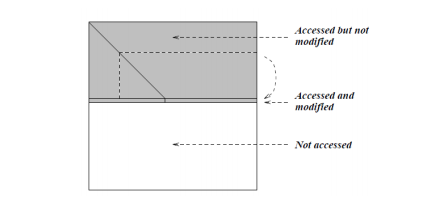
\includegraphics[width=0.7\linewidth]{figures/Figure_6.png}  %插入的图,包括JPG,PNG,PDF,EPS等,放在源文件目录下
	\caption{}  %图片的名称
	\label{fig:mcmthesis-logo}   %标签,用作引用
\end{figure}

\begin{framed}	
思考:如果数据按列存储, 如 FORTRAN/MATLAB, 如何设计算法?	
\end{framed}

\subsubsection{待定系数法计算 LU 分解}

设 $A = LU$, 即

{$\left[\begin{array}{ccccc}{a_{11}} & {a_{12}} & {a_{13}} & {\cdots} & {a_{1 n}} \\ {a_{21}} & {a_{22}} & {a_{23}} & {\cdots} & {a_{2 n}} \\ {a_{31}} & {a_{32}} & {a_{33}} & {\cdots} & {a_{3 n}} \\ {\vdots} & {} & {} & {\ddots} & {\vdots} \\ {a_{n 1}} & {a_{x 2}} & {a_{x 3}} & {\cdots} & {a_{n n}}\end{array}\right]$ =$\left[\begin{array}{cccc}{1} & {} & {} & {} \\ {l_{21}} & {1} & {} & {} \\ {l_{31}} & {l_{32}} & {1} & {} \\ {\vdots} & {} & {} & {\ddots} \\ {l_{n 1}} & {l_{n 2}} & {\cdots} & {l_{n, n-1}}\end{array}\right]$$ \left[\begin{array}{ccccc}{u_{11}} & {u_{12}} & {u_{13}} & {\cdots} & {u_{1 n}} \\ {} & {u_{22}} & {u_{23}} & {\cdots} & {u_{2 n}} \\ {} & {} & {u_{33}} & {\cdots} & {u_{2 n}} \\ {} & {} & {} & {\ddots} & {\vdots} \\ {} & {} & {} & {} & {u_{n n i}}\end{array}\right] $}

\noindent(1)比较等式两边的第一行, 可得

$u_{1 j}=a_{1 j}, \quad j=1,2, \dots, n$

再比较等式两边的第一列, 可得

$a_{i 1}=l_{i 1} u_{11} \Rightarrow l_{i 1}=a_{i 1} / u_{11}, \quad i=2,3, \ldots, n$

\noindent(2) 比较等式两边的第二行, 可得

$a_{2 j}=l_{21} u_{1 j}+a_{2 j} \Rightarrow u_{2 j}=a_{2 j}-l_{21} u_{1 j}, \quad j=2,3, \ldots, n$

再比较等式两边的第二列, 可得

$a_{i 2}=l_{i 1} u_{12}+l_{i 2} u_{22} \Rightarrow l_{i 1}=\left(a_{i 2}-l_{i 1} u_{12}\right) / u_{22}, \quad i=3,4, \ldots, n$

\noindent(3) 以此类推, 第 k 步时, 比较等式两边的第 k 行, 可得

$u_{k j}=a_{k j}-\left(l_{k 1} u_{1 j}+\cdots+l_{k, k-1} u_{k-1, j}\right), \quad j=k, k+1, \ldots, n$

比较等式两边的第 k 列, 可得

$l_{i k}=\left(a_{i k}-l_{i 1} u_{1 k}-\cdots-l_{i, k-1} u_{k-1, k}\right) / u_{k k}, \quad i=k+1, k+2, \ldots, n$

直到第 n 步, 即可计算出 L 和 U 的所有元素.

同样, 我们可以利用 A 来存储 L 和 U. 算法描述如下:
\begin{table}  
	%\caption{设置表格总长}  
	\begin{tabular*}{16cm}{ll}  
		\hline  
		算法 4.5 &LU 分解 (待定系数法或 $Doolittle$ 方法)\\  
		\hline  
		1:   & for k = 1 to n do\\  
		2:   & \qquad $a_{k j}=a_{k j}-\sum_{i=1}^{k-1} a_{k i} a_{i j}, \quad j=k, k+1, \ldots, n$\\
		3:   & \qquad $a_{i k}=\frac{1}{a_{k k}}\left(a_{i k}-\sum_{j=1}^{k-1} a_{i j} a_{j k}\right), \quad i=k+1, k+2, \ldots, n$\\
		4:   & end for\\
		\hline  
	\end{tabular*}  
\end{table} 

\begin{lstlisting}[language={[ANSI]C}] 
% Matlab code 2 : 待定系数法 LU 分解
function A = mylu2(A)
[n,n]=size(A);
for k=1:n
A(k,k)=A(k,k)-A(k,1:k-1)*A(1:k-1,k);
if (A(k,k)==0)
fprintf('Error: A(%d,%d)=0!\n', i,i);
return;
end
A(k,k+1:n)=A(k,k+1:n)-A(k,1:k-1)*A(1:k-1,k+1:n);
A(k+1:n,k)=A(k+1:n,k)-A(k+1:n,1:k-1)*A(1:k-1,k);
A(k+1:n,k)=A(k+1:n,k)/A(k,k);
end
\end{lstlisting}

\subsubsection{三角方程求解}
得到 $A$ 的 $LU$ 分解后, 我们最后需要用回代法求解两个三角方程组
$$L y=b, \quad U x=y$$

\begin{table}  
	%\caption{设置表格总长}  
	\begin{tabular*}{16cm}{ll}  
		\hline  
		算法 4.6 &向前回代求解$Ly =b$(假定$L$是一般的非奇异下三角矩阵)\\  
		\hline  
		1:   &$y_{1}=b_{1} / l_{11}$\\  
		2:   & for i = 2 : n do\\
		3:   & \qquad for j = 1 : i − 1 do\\
		4:    & \qquad \qquad$b_{i}=b_{i}-l_{i j} y_{j}$\\
		5:   & \qquad end for\\
		6:    & \qquad $y_{i}=b_{i} / l_{i i}$\\
		7:    & end for\\
		\hline  
	\end{tabular*}  
\end{table}

如果数据是按列存储的, 则采用列存储方式效率会高一些.

下面是按列存储方式求解上三角方程组.

\begin{table}  
	%\caption{设置表格总长}  
	\begin{tabular*}{16cm}{ll}  
		\hline  
		算法 4.7 &向前回代求解$Ly =b$(假定$L$是一般的非奇异下三角矩阵)\\  
		\hline  
		1:   & for i = n : −1 : 1 do\\  
		2:   & \qquad $x_{i}=y_{i} / u_{i i}$\\
		3:   & \qquad for j = i − 1 : −1 : 1 do\\
		4:    & \qquad \qquad$y_{j}=y_{j}-x_{i} u_{j i}$\\
		5:   & \qquad end for\\
		6:    & end for\\
		\hline  
	\end{tabular*}  
\end{table}

这两个算法的运算量均为$n^2+O(n)$

\subsubsection{选主元 LU 分解}
• 在 LU 分解算法 1.2 中, 我们称 $a_{k k}^{(k-1)}$ 为主元. 如果 $a_{k k}^{(k-1)}=0$, 则算法就无法进行下去.

• 即使 $a_{k k}^{(k-1)}$ 不为零, 但如果$\left|a_{k k}^{(k-1)}\right|$ 的值很小, 由于舍入误差的原因,也可能会给计算结果带来很大的误差.

• 此时我们就需要通过 选主元 来解决这个问题.

\begin{framed}
\bfseries{例} 用 LU 分解求解线性方程组 Ax = b, 其中
	\begin{equation}
	A=\left[\begin{array}{cc}{0.02} & {61.3} \\ {3.43} & {-8.5}\end{array}\right], \quad b=\left[\begin{array}{c}{61.5} \\ {25.8}\end{array}\right]
	\end{equation}

要求在运算过程中保留 3 位有效数字.	

$(x_1 ≈ −20.7, x_2 ≈ 1.01)$
\end{framed}

易知, 方程的精确解为 $x_1 = 10.0$ 和 $x_2 = 1.00$. 我们发现 $x_1$ 的误差非常
大. 导致这个问题的原因就是 $|a_{11}| $太小, 用它做主元时会放大舍入误差.
所以我们需要选主元.

\subsection{选主元 LU 分解}
\begin{framed}
\begin{theorem}
	设 $A ∈ R^{n×n}$ 非奇异, 则存在置换矩阵 $P_L$,$ P_R$, 以及单位下三角
	矩阵 $L$ 和非奇异上三角矩阵 $U$, 使得 $P_LAP_R = LU$. 其中 $P_L$ 和 $P_R$ 中只有一个是必需的.
\end{theorem}
\end{framed}

第 $k$ 步时, 如何选取置换矩阵 $P^{(k)}_L$ 和 $P^{(k)}_R$ ?

选法一. 选取 $P^{(k)}_L$ 和 $P^{(k)}_R$ 使得主元为剩下的矩阵中绝对值最大, 这种选
取方法称为 “全主元 $Gauss$ 消去法”, 简称 $GECP$ (Gaussian elimination
with complete pivoting);

选法二. 选取 $P^{(k)}_L$ 和$ P^{(k)}_R$ 使得主元为第 $k$ 列中第 $k$ 到第 $n$ 个元素中, 绝对值最大, 这种选取方法称为 “部分选主元 $Gauss$ 消去法”, 简称 $GEPP$
(Gaussian elimination with partial pivoting), 此时 $P^{(k)}_R = I$, 因此也称为列主元 $Gauss$ 消去法.

\begin{framed}
	† (1) $GECP$ 比 $GEPP$ 更稳定, 但工作量太大, 在实际应用中通常使用
	$GEPP$ 算法.
	(2) $GEPP$ 算法能保证$L$ 所有的元素的绝对值都不超过 $1$.
\end{framed}

\begin{table}  
	%\caption{设置表格总长}  
	\begin{tabular*}{16cm}{ll}  
		\hline  
		算法 4.7 &向前回代求解$Ly =b$(假定$L$是一般的非奇异下三角矩阵)\\  
		\hline  
		1:   & p = 1 : n \% 用于记录置换矩阵\\  
		2:   & for k = 1 to n − 1 do\\
		3:   & \qquad $\left[a_{\max }, l\right]=\max _{k \leq i \leq n}\left|a_{i k}\right|$ \% 选列主元, 其中 l 表示主元所在的行 \\
		4:    & \qquad if l ̸= k then\\
		5:   & \qquad \qquad for j = 1 to n do\\
		6:    & \qquad \qquad \qquad $t m p=a_{k j}, a_{k j}=a_{l j}, a_{l j}=\operatorname{tm} p$ \% 交换第 k 行与第l 行\\
		7:    &\qquad \qquad end for\\
		8:   & \qquad \qquad $\operatorname{tm} p=p(k), p(k)=p(l), p(l)=\operatorname{tm} p$ \%更新置换矩阵 \\
		9:   & \qquad end if\\
	   10:   & \qquad for i = k + 1 to n do\\
	   11:   & \qquad \qquad $a_{i k}=a_{i k} / a_{k k}$ \%计算 L 的第 k 列\\
	   12:   & \qquad end for\\
	   13:   & \qquad for i = k + 1 to n do\\
	   14:   & \qquad \qquad for j = k + 1 to n do\\
	   15:   & \qquad \qquad \qquad $a_{i j}=a_{i j}-a_{i k} * a_{k j}$ \%更新 A(k + 1 : n, k + 1 : n) \\
	   16:   & \qquad \qquad end for \\
	   17:   & \qquad end for \\
	   18:    & end for \\
		\hline  
	\end{tabular*}  
\end{table}

\begin{lstlisting}[language={[ANSI]C}] 
% Matlab code 2 : 部分选主元 LU 分解
function [A,p] = myplu(A)
[n,n]=size(A); p=1:n;
for i=1:n-1
[a,k]=max(abs(A(i:n,i)));
if a==0
error('Error: 第 %d 步的列主元为 0!\n', i);
end
k=k+i-1;
if k~=i
tmp=A(i,:); A(i,:)=A(k,:); A(k,:)=tmp;
tmp=p(i); p(i)=p(k); p(k)=tmp;
end
A(i+1:n,i)=A(i+1:n,i)/A(i,i);
A(i+1:n,i+1:n)=A(i+1:n,i+1:n)-A(i+1:n,i)*A(i,i+1:n);
end
\end{lstlisting}

\begin{framed}
	\bfseries{例} 用 LU 分解求解线性方程组 Ax = b, 其中
	\begin{equation}
	A=\left[\begin{array}{cc}{0.02} & {61.3} \\ {3.43} & {-8.5}\end{array}\right], \quad b=\left[\begin{array}{c}{61.5} \\ {25.8}\end{array}\right]
	\end{equation}
	
	要求在运算过程中保留 3 位有效数字.	
	
	$(x_1 ≈ 10.0, x_2 ≈ 0.998)$
\end{framed}

\subsubsection{矩阵求逆}
我们可以通过部分选主元 $LU$ 分解来计算矩阵的逆. 设 $P A = LU$, 则

$$
A^{-1}=P^{T} U^{-1} L^{-1}
$$

等价于求解下面 $2n$ 个三角线性方程组

$$
L y_{i}=P e_{i}, \quad U x_{i}=y_{i}, \quad i=1,2, \ldots, n
$$

也可以分别计算 $L^{-1}$ 和 $U^{−1}$, 然后相乘. 哪种方法划算?

\subsection{特殊方程组的求解}

2.1 对称正定线性方程组

2.2 对称不定线性方程组

2.3 三对角线性方程组

2.4 带状线性方程组

2.5 Toeplitz 线性方程组

\subsubsection{对称正定线性方程组}

我们首先给出对称正定矩阵的几个基本性质.
\begin{framed}
	\begin{theorem}
		设$ A ∈ \mathbb{R}^{n×n}$.
		• $A$ 对称正定当且仅当 $A$ 对称且所有特征值都是正的;
		
		• $A $对称正定当且仅当 $X^{⊺}AX$ 对称正定, 其中 $X ∈ \mathbb{R}^{n×n} $是一个任意的非奇异矩阵;
		
		• 若 $A$ 对称正定, 则 $A$ 的任意主子矩阵都对称正定;
		
		• 若 $A$ 对称正定, 则 $A$ 的所有对角线元素都是正的, 且
		$$
		\max _{i \neq j}\left\{\left|a_{i j}\right|\right\}<\max _{i}\left\{a_{i i}\right\}
		,$$即绝对值最大的元素出现在对角线上.
	\end{theorem}
\end{framed}

{\bfseries Cholesky 分解}

\begin{framed}
	\begin{theorem}(Cholesky 分解)
	设 $A ∈ \mathbb{R}^{n×n}$ 对称正定, 则存在唯一的对角线元
	素为正的下三角矩阵$ L$, 使得
	$$
	A=L L^{\top}
	$$
	该分解称为 $Cholesky$ 分解.	
	\end{theorem}
\end{framed}

{\bfseries Cholesky 分解的实现}
设 $A = LL^{⊺}$, 即
\begin{equation}
\left[\begin{array}{cccc}{a_{11}} & {a_{12}} & {\cdots} & {a_{1 n}} \\ {a_{21}} & {a_{22}} & {\cdots} & {a_{2 n}} \\ {\vdots} & {} & {\ddots} & {\vdots} \\ {a_{n 1}} & {a_{n 2}} & {\cdots} & {a_{n n}}\end{array}\right]=\left[\begin{array}{cccc}{l_{11}} & {} & {} & {} \\ {l_{21}} & {l_{22}} & {} & {} \\ {\vdots} & {\vdots} & {\ddots} & {} \\ {l_{n 1}} & {l_{n 2}} & {\cdots} & {l_{n n}}\end{array}\right]\left[\begin{array}{cccc}{l_{11}} & {l_{21}} & {\cdots} & {l_{n 1}} \\ {} & {l_{22}} & {\cdots} & {l_{n 2}} \\{}& {} & {\ddots} & {\vdots} \\{} &{} & {} & {l_{n n}}\end{array}\right]
\end{equation}

直接比较等式两边的元素可得
\begin{equation}
a_{i j}=\sum_{k=1}^{n} l_{i k} l_{j k}=l_{j j} l_{i j}+\sum_{k=1}^{j-1} l_{i k} l_{j k}, \quad i, j=1,2, \ldots, n
\end{equation}

根据上面的计算公式, 可得下面的算法:

\begin{table}  
	%\caption{设置表格总长}  
	\begin{tabular*}{16cm}{ll}  
		\hline  
		算法 4.8 & Cholesky 分解算法\\  
		\hline  
		1:   & for j = 1 to n do\\  
		2:   & \qquad $l_{j j}=\left(a_{j j}-\sum_{k=1}^{j-1} l_{j k}^{2}\right)^{1 / 2}$\\
		3:   & \qquad for i = j + 1 to n do\\
		4:    & \qquad \qquad$l_{i j}=\left(a_{i j}-\sum_{k=1}^{j-1} l_{i k} l_{j k}\right) / l_{j j}$\\
		5:   & \qquad end for\\
		6:    & end for\\
		\hline  
	\end{tabular*}  
\end{table}

{\bfseries 几点说明}

• 与 $LU$ 分解一样, 可以利用 $A$ 的下三角部分来存储 $L$;

• $Cholesky$ 分解算法的运算量为$\frac{1}{3} n^{3}+O\left(n^{2}\right)$, 大约为 $LU$ 分解的一半;

• $Cholesky$ 分解算法是稳定的(稳定性与全主元 $Gauss$ 消去法相当),
故不需要选主元.

{\bfseries 改进的 Cholesky 分解算法}
为了避免开方运算, 我们可以将 $A$ 分解为: $A = LDL^{\top}$, 即
\begin{equation}
\left[\begin{array}{cccc}{a_{11}} & {a_{12}} & {\cdots} & {a_{1 n}} \\ {a_{21}} & {a_{22}} & {\cdots} & {a_{2 n}} \\ {\vdots} & {} & {\ddots} & {\vdots} \\ {a_{n 1}} & {a_{n 2}} & {\cdots} & {a_{n n}}\end{array}\right]=\left[\begin{array}{cccc}{1} & {} & {} & {} \\ {l_{21}} & {1} & {} & {} \\ {\vdots} & {} & {\ddots} & {} \\ {l_{n 1}} & {\cdots} & {l_{n, n-1}} & {1}\end{array}\right]\left[\begin{array}{cccc}{d_{1}} & {} & {} & {} \\ {} & {d_{2}} & {} & {} \\ {} & {} & {\ddots} & {} \\ {} & {} & {} & {d_{n}}\end{array}\right]\left[\begin{array}{cccc}{1} & {l_{21}} & {\cdots} & {l_{n 1}} \\ {1} & {\cdots} & {l_{n 2}} \\ {} & {\ddots} & {\vdots} \\ {} & {} & {1}\end{array}\right]
\end{equation}

通过待定系数法可得
\begin{equation}
a_{i j}=\sum_{k=1}^{n} l_{i k} d_{k} l_{j k}=d_{j} l_{i j}+\sum_{k=1}^{j-1} l_{i k} d_{k} l_{j k}, \quad i, j=1,2, \ldots, n
\end{equation}

基于以上分解来求解对称正定线性方程组的算法称为改进的平方根法:
\begin{table}  
	%\caption{设置表格总长}  
	\begin{tabular*}{16cm}{ll}  
		\hline  
		算法 4.9 &改进的平方根法\\  
		\hline  
		1:   & for j = 1 to n do \% 先计算分解\\  
		2:   & \qquad $d_{j}=a_{j j}-\sum_{k=1}^{j-1} l_{j k}^{2} d_{k}$\\
		3:   & \qquad for i = j + 1 to n do \\
		4:    & \qquad $l_{i j}=\left(a_{i j}-\sum_{k=1}^{j-1} l_{i k} d_{k} l_{j k}\right) / d_{j}$\\
		5:   & \qquad end for\\
		6:    & end for\\
		7:    & $y_1 = b_1$ \% 解方程组: Ly = b 和 $DL^{\top}x = y$\\
		8:   & for i = 2 to n do \\
		9:   & \qquad $y_{i}=b_{i}-\sum_{k=1}^{i-1} l_{i k} y_{k}$\\
		10:   & end for\\
		11:   & $x_{n}=y_{n} / d_{n}$\\
		12:   & for i = n − 1 to 1 do\\
		13:   & \qquad $x_{i}=y_{i} / d_{i}-\sum_{k=i+1}^{n} l_{k i} x_{k}$\\
		14:   & end for\\
		\hline  
	\end{tabular*}  
\end{table}

\subsubsection{对称不定线性方程组}

$A → $非奇异, 对称不定

若 $A$ 存在 $LU$ 分解, 即 $A = LU$, 则可写成 $A = LDL^{\top}$

然而, 当 $A$ 不定时, 其 $LU$ 分解不一定存在.

若采用选主元 $LU$ 分解, 则其对称性将被破坏. 为了保持对称性, 在选主元
时必须对行列进行同样的置换, 即选取置换矩阵 $P$, 使得

\begin{equation}
P A P^{\top}=L D L^{\top}
\end{equation}

通常称 (2.4) 为对称矩阵的 $LDL^{\top}$ 分解.

不幸的是, 这样的置换矩阵可能不一定存在, 即分解 (2.4) 不一定存在.


\begin{framed}
{\bfseries 例} 设对称矩阵

\begin{equation}
A=\left[\begin{array}{lll}{0} & {1} & {1} \\ {1} & {0} & {1} \\ {1} & {1} & {0}\end{array}\right]
\end{equation}

由于 $A$ 的对角线元素都是 $0$, 对任意置换矩阵 $P$, 矩阵 $P AP^{\top}$ 的对角线
元素仍然都是 $0$. 因此, 矩阵 $A$ 不存在 $LDL^{\top}$ 分解.

\end{framed}

{\bfseries Aasen 算法}

1971 年, Aasen 提出了下面的分解

\begin{equation}
P A P^{\top}=L T L^{\top}
\end{equation}

其中 $P$ 为置换矩阵, $L$ 为单位下三角矩阵, $T$ 为对称三对角矩阵.

分解 (2.5) 本质上与部分选主元 LU 分解是一样的.

{\bfseries 块 $LDL^{\top}$ 分解} 

设 $A$ 对称非奇异, 则存在置换矩阵 $P$ 使得
\begin{equation}
P A P^{\top}=\left[\begin{array}{cc}{B} & {E^{\top}} \\ {E} & {C}\end{array}\right]
\end{equation}
其中 $B ∈ \mathbb{R}$ 或 $B ∈ \mathbb{R}^{2×2}$
, 且非奇异. 因此可以对 $P AP^{\top}$ 进行块对角化, 即

\begin{equation}
P A P^{\top}=\left[\begin{array}{cc}{I} & {0} \\ {E B^{-1}} & {I}\end{array}\right]\left[\begin{array}{cc}{B} & {0} \\ {0} & {C-E B^{-1} E^{\top}}\end{array}\right]\left[\begin{array}{cc}{I} & {B^{-1} E^{\top}} \\ {0} & {I}\end{array}\right]
\end{equation}

其中$C-E B^{-1} E^{\top}$是$Schur$补。

不断重复以上过程, 就可以得到 A 的块 $LDL^{\top}$ 分解:
\begin{equation}
P A P^{\top}=L \tilde{D} L^{\top}
\end{equation}
其中$\tilde{D}$是拟对角矩阵, 即块对角矩阵且对角块的大小为 1 或 2

{\bfseries 选主元块 $LDL^{\top}$ 分解}
与选主元 $LU$ 分解类似, 我们需要考虑块 $LDL^{\top}$ 分解的选主元策略, 即如何
选取置换矩阵. 目前常用的策略有

• 全主元策略: 由 $Bunch$ 和 $Parlett$ 于 1971 年提出, 并证明了其稳定性.
但需要进行 $n^3/6$ 次比较运算, 代价比较昂贵.

• 部分选主元策略: 由 $Bunch$ 和 $Kaufman$ 于 1977 年提出, 将比较运算
复杂度降低到 $O(n^2)$ 量级, 而且具有较满意的向后稳定性. 因此被广
泛使用.

• Rook 策略: 由 Ashcraft, Grimes 和 Lewis 于 1998 年提出, 整体上与部
分选主元类似, 但在选主元时加了一层迭代, 从而能提供更高的精度

\begin{framed}
	目前大部分软件都采用部分选主元块 $LDL^{\top}$分解算法
\end{framed}

\subsubsection{三对角线性方程组}
\begin{equation}
A=\left[\begin{array}{cccc}{b_{1}} & {c_{1}} & {} & {} \\ {a_{1}} & {\ddots} & {\ddots} & {} \\ {} & {\ddots} & {\ddots} & {c_{n-1}} \\ {} & {} & {a_{n-1}} & {b_{n}}\end{array}\right]
\end{equation}
我们假定

\begin{equation}
\left|b_{1}\right|>\left|c_{1}\right|>0, \quad\left|b_{n}\right|>\left|a_{n-1}\right|>0
\end{equation}
\begin{equation}
\left|b_{i}\right| \geq\left|a_{i-1}\right|+\left|c_{i}\right|, \quad a_{i} c_{i} \neq 0, \quad i=1, \ldots, n-1
\end{equation}

即 A 是 不可约弱对角占优

\begin{framed}
	如果 A 可约, 怎么处理?
\end{framed}

此时, 我们可以得到下面的三角分解
\begin{equation}
A=\left[\begin{array}{cccc}{b_{1}} & {c_{1}} & {} & {} \\ {a_{1}} & {\ddots} & {\ddots} & {} \\ {} & {\ddots} & {\ddots} & {c_{n-1}} \\ {} & {} & {a_{n-1}} & {b_{n}}\end{array}\right]=\left[\begin{array}{cccc}{\alpha_{1}} & {} & {} & {} \\ {a_{1}} & {\alpha_{2}} & {} & {} \\ {} & {\ddots} & {\ddots} & {} \\ {} & {} & {a_{n-1}} & {\alpha_{n}}\end{array}\right]\left[\begin{array}{cccc}{1 \beta_{1}} \\ {1} & {\ddots} \\ {} & {\ddots} & {\beta_{n-1}} \\ {} & {} & {1}\end{array}\right] \triangleq L U
\end{equation}

递推公式:
\begin{equation}
\begin{array}{l}{\alpha_{1}=b_{1}} 
\\ {\beta_{1}=c_{1} / \alpha_{1}=c_{1} / b_{1}} 
\\ {\left\{\begin{array}{l}{\alpha_{i}=b_{i}-a_{i-1} \beta_{i-1}} \\ {\beta_{i}=c_{i} / \alpha_{i}=c_{i} /\left(b_{i}-a_{i-1} \beta_{i-1}\right), \quad i=2,3, \ldots, n-1} \end{array}\right.}\\ {\alpha_{n}=b_{n}-a_{n-1} \beta_{n-1}}\end{array}
\end{equation}

为了使得算法能够顺利进行下去, 我们需要证明$\alpha_{i} \neq 0$

\begin{framed}
	\begin{theorem}
		设三对角矩阵 A 满足条件 (2.6) 和 (2.7). 则 A 非奇异, 且
	    
	    (1)$\left|\alpha_{1}\right|=\left|b_{1}\right|>0$
	    
	    (2) $0<\left|\beta_{i}\right|<1, i=1,2, \ldots, n-1$
	    
	    (3)	$0<\left|c_{i}\right| \leq\left|b_{i}\right|-\left|a_{i-1}\right|<\left|\alpha_{i}\right|<\left|b_{i}\right|+\left|a_{i-1}\right|, i=2,3, \ldots, n$
	\end{theorem}
\end{framed}

\begin{table}  
	%\caption{设置表格总长}  
	\begin{tabular*}{16cm}{ll}  
		\hline  
		算法 4.9 &改进的平方根法\\  
		\hline  
		1:   & $\beta_{1}=c_{1} / b_{1}$\\  
		2:   & $y_{1}=f_{1} / b_{1}$\\
		3:   & : for i = 2 to n−1 do \\
		4:    & \qquad $\alpha_{i}=b_{i}-a_{i-1} \beta_{i-1}$\\
		5:   & \qquad $\beta_{i}=c_{i} / \alpha_{i}$\\
		6:    & \qquad $y_{i}=\left(f_{i}-a_{i-1} y_{i-1}\right) / \alpha_{i}$\\
		7:   & end for\\
		8:   & $\alpha_{n}=b_{n}-a_{n-1} \beta_{n-1}$ \\
		9:   & $y_{n}=\left(f_{n}-a_{n-1} y_{n-1}\right) / \alpha_{n}$\\
		10:  & $x_{n}=y_{n}$\\
		11:  & for i = n−1 to 1 do\\
		12:  & \qquad $x_{i}=y_{i}-\beta_{i} x_{i+1}$\\
		13:  & end for\\
		\hline  
	\end{tabular*}  
\end{table}

\begin{framed}
	† 追赶法 (也称为 Thomas 算法) 的运算量大约为 $8n − 6$.
\end{framed}

\begin{framed}
	† 具体计算时, 由于求解 $Ly = f$ 与矩阵 $LU$ 分解是同时进行的, 因此,
	$\alpha_i$ 可以不用存储. 但 $\beta_i$ 需要存储.
\end{framed}

\begin{framed}
	† 由于 $|\beta_i| < 1$, 因此在回代求解 $x_i$ 时, 误差可以得到有效控制.
\end{framed}

需要指出的是, 我们也可以考虑下面的分解
\begin{equation}
A=\left[\begin{array}{cccc}{b_{1}} & {c_{1}} & {} & {} \\ {a_{1}} & {\ddots} & {\ddots} & {} \\ {} & {\ddots} & {\ddots} & {c_{n-1}} \\ {} & {} & {a_{n-1}} & {b_{n}}\end{array}\right]=\left[\begin{array}{ccccc}{1} \\ {\gamma_{1}} & {1} & {} & {} \\ {} & {\ddots} & {\ddots} & {} \\ {} & {} & {\gamma_{n-1}} & {1}\end{array}\right]\left[\begin{array}{cccc}{\alpha_{1}} & {c_{1}} & {} & {} \\ {} & {\alpha_{2}} & {\ddots} & {} \\ {} & {} & {\ddots} & {c_{n-1}} \\ {} & {} & {} & {\alpha_{n}}\end{array}\right]
\end{equation}

但此时$ |\gamma_i|$ 可能大于 1. 比如$ \gamma_1 = a_1/b_1$, 因此当$|b_1| < |a_1|$ 时, $|\gamma_1| > 1$.
所以在回代求解时, 误差可能得不到有效控制. 另外一方面, 计算$ γi$ 时也
可能会产生较大的舍入误差 (大数除以小数).

但如果 A 是列对角占优, 则可以保证$ |\gamma_i| < 1.$

\begin{framed}
† 如果 A 是 (行) 对角占优, 则采用前面的分解;
	
如果 A 是列对角占优, 则采用分解 (2.11).
\end{framed}

\subsubsection{带状线性方程组}
设 $A ∈ R^{n×n}$ 是带状矩阵, 其下带宽为 $b_L$, 上带宽为$b_U$ , 即
\begin{equation}
a_{i j}=0 \quad \text { for } \quad i>j+b_{L} \text { or } i<j-b_{U}
\end{equation}

\begin{figure}[h]%%图
	\centering  %插入的图片居中表示
	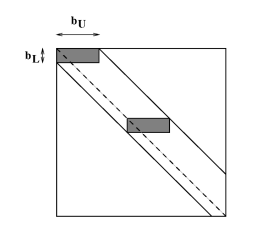
\includegraphics[width=0.7\linewidth]{figures/Figure_7.png}  %插入的图,包括JPG,PNG,PDF,EPS等,放在源文件目录下
	\caption{}  %图片的名称
	\label{fig:mcmthesis-logo}   %标签,用作引用
\end{figure}

对于带状矩阵, 其 LU 分解有如下性质:
\begin{framed}
	\begin{theorem}
	设 $A ∈ R^{n×n}$ 是带状矩阵, 其下带宽为 $b_L$, 上带宽为 $b_U$ . 若 $A =
	L_U$ 是不选主元的 $L_U$ 分解, 则 $L$ 为下带宽为 $b_L$ 的带状矩阵, $U$ 为上带
	宽为 $b_U$ 的带状矩阵.	
	\end{theorem}
\end{framed}

统计求解带状矩阵 $Ax = b$ 的运算量.

若采用部分选主元的 LU 分解, 则有
\begin{framed}
	\begin{theorem}
		设 $A ∈ R
		n×n $是带状矩阵, 其下带宽为$ b_L$, 上带宽为 $b_U$ . 若 $P A =
		LU $是部分选主元的 $LU$ 分解, 则 $U$ 为上带宽不超过$b_L + b_U$ 的带状矩
		阵, $L $为下带宽为 $b_L$ 的 “基本带状矩阵”, 即 L 每列的非零元素不超过
		$b_L + 1$ 个.
	\end{theorem}
\end{framed}

\subsubsection{Toeplitz 线性方程组}
\begin{equation}
T_{n}=\left[\begin{array}{cccc}{t_{0}} & {t_{-1}} & {\cdots} & {t_{-n+1}} \\ {t_{1}} & {\ddots} & {\ddots} & {\vdots} \\ {\vdots} & {\ddots} & {\ddots} & {t_{-1}} \\ {t_{n-1}} & {\cdots} & {t_{1}} & {t_{0}}\end{array}\right]
\end{equation}
$T_n$ 是反向对称 (persymmetric) 矩阵. 记 $J_n $为$ n$ 阶反向单位矩阵:
\begin{equation}
J_{n}=\left[\begin{array}{cccc}{ } & { } & { } &{1} \\{ } & { } &{1} & { } \\ {} & {\cdots}& { } & { } \\ {1} &{ } &{ } &{ }\end{array}\right]
\end{equation}
易知$J_{n}^{\top}=J_{n}^{-1}=J_{n}$

\begin{framed}
	\begin{lemma}
		矩阵$ A ∈ \mathbb{R}^{n×n}$ 是反向对称矩阵当且仅当
			\begin{equation}
			A=J_{n} A^{\top} J_{n} \quad \text { 或 } \quad J_{n} A=A^{\top} J_{n}
			\end{equation}
	\end{lemma}
\end{framed}

若 A 可逆, 则可得
\begin{equation}
A^{-1}=J_{n}^{-1}\left(A^{\top}\right)^{-1} J_{n}^{-1}=J_{n}\left(A^{-1}\right)^{\top} J_{n}
\end{equation}

即反向对称矩阵的逆也是反向对称矩阵.
\begin{framed}
	† Toeplitz 矩阵的逆是反向对称矩阵, 但不一定是 Toeplitz 矩阵.
\end{framed}

{\bfseries Yule-Walker 方程组}

假定 $T_n$ 对称正定, 考虑线性方程组
\begin{equation}
T_{n} x=-r_{n}
\end{equation}

其中 $r_n = [t_1, t_2, . . . , t_{n−1}, t_n]^{\top}$
. 这类线性方程组称为 $Yule-Walker$ 方程组,
其中 $t_n$ 为任意给定的实数.

由于 $T_n$ 对称正定, 所以 $t_0 > 0$. 因此我们可以对 $T_n$ 的对角线元素进行单位化. 不失一般性, 我们假定 $T_n$ 的对角线元素为 1, 即
\begin{equation}
T_{n}=\left[\begin{array}{cccc}{1} & {t_{1}} & {\cdots} & {t_{n-1}} \\ {t_{1}} & {\ddots} & {\ddots} & {\vdots} \\ {\vdots} & {\ddots} & {\ddots} & {t_{1}} \\ {t_{n-1}} & {\cdots} & {t_{1}} & {1}\end{array}\right]
\end{equation}

由于方程组右端项的特殊性, 我们可以通过递推来求解.

记$T_{k} x=-r_{k}$的解为$\mathcal{X}^{(k)}$.设$T_{k+1} x=-r_{k+1}$的解$x^{(k+1)}=\left[\begin{array}{c}{z^{(k)}} \\ {\alpha_{k}}\end{array}\right]$。

代入后可得递推公式:
\begin{framed}
	\begin{equation}
	\alpha_{k}=\frac{-t_{k+1}-r_{k}^{\top} J_{k} x^{(k)}}{1+r_{k}^{\top} x^{(k)}}, \quad z^{(k)}=x^{(k)}+\alpha_{k} J_{k} x^{(k)} \quad k=1,2, \ldots
	\end{equation}
\end{framed}

因此, 我们就可以从一阶 $Yule-Walker$ 方程出发, 利用递推公式 (2.13) 计算
$T_nx = −r_n $的解. 总的运算量 (乘法与加减运算) 大约为 $3n^2$
.

为了减少运算量, 我们引入一个变量$\beta_{k} \triangleq 1+r_{k}^{\top} x^{(k)}$,则:
\begin{equation}
\begin{aligned} \beta_{k+1} &=1+r_{k+1}^{\top} x^{(k+1)} \\ &=1+\left[r_{k}^{\top}, t_{k+1}\right]\left[\begin{array}{c}{x^{(k)}+\alpha_{k} J_{k} x^{(k)}} \\ {\alpha_{k}}\end{array}\right] \\ &=1+r_{k}^{\top} x^{(k)}+\alpha_{k}\left(t_{k+1}+r_{k}^{\top} J_{k} x^{(k)}\right) \\ &=\left(1-\alpha_{k}^{2}\right) \beta_{k} \end{aligned}
\end{equation}

总运算量降为 $2n^2$
. 这就是求解 Yule-Walker 方程组的 Durbin 算法.

\begin{table}  
	%\caption{设置表格总长}  
	\begin{tabular*}{16cm}{ll}  
		\hline  
		算法  &求解 Yule-Walker 方程组的 Durbin 算法\\  
		\hline  
		1:   & 输入数据: $t = [t_1, t_2, . . . , t_n]$ \% 注: 这里假定 t0 = 1\\  
		2:   & $x(1) = −t_1, β = 1, α = −t_1$\\
		3:   & for for k = 1 to n − 1 do \\
		4:    & \qquad $\beta=(1-\alpha^2)\beta$\\
		5:   & \qquad $\alpha=-\left(t_{k+1}-\sum_{i=1}^{k} t_{k+1-i} x(i)\right) / \beta$\\
		6:    & \qquad $x(1 : k)=x(1 : k)+\alpha x(k :-1 : 1)$\\
		7:   &$x(k+1)=\alpha$\\
		8:   & end for\\
		\hline  
	\end{tabular*}  
\end{table}


{\bfseries 一般右端项的对称正定 Toeplitz 线性方程组}

考虑一般右端项的方程组 $T_nx = b$ , 其中 $T_n$ 对称正定.

我们利用递推方法来求解: 假定 $x^{(k)}$ 和 $y^{(k)}$ 分别是下面两个方程组的解:

\begin{equation}
T_{k} x=\left[b_{1}, b_{2}, \ldots, b_{k}\right]^{\top}, \quad T_{k} y=-\left[t_{1}, t_{2}, \ldots, t_{k}\right]^{\top}
\end{equation}

设$x^{(k+1)}=\left[\begin{array}{c}{z^{(k)}} \\ {\mu_{k}}\end{array}\right]$是$T_{k+1} x=b^{(k+1)}$的解,则可得

\begin{equation}
z^{(k)}=x^{(k)}+\mu_{k} J_{k} y^{(k)}, \quad \mu_{k}=\frac{b_{k+1}-r_{k}^{\top} J_{k} x^{(k)}}{1+r_{k}^{\top} y^{(k)}}
\end{equation}

所以, 我们可以先计算$T_{k} x=b^{(k)}$和$T_{k} x=-r_{k}$的解,, 然后利用上述公式得到$T_{k+1} x=b^{(k+1)}$的解,这就是 Levinson 算法, 总运算量大约为 $4n^2$.

\begin{table}  
	%\caption{设置表格总长}  
	\begin{tabular*}{16cm}{ll}  
		\hline  
		算法 4.9 &求解对称正定 Toeplitz 线性方程组的 Levinson 算法\\  
		\hline  
		1:   & 输入数据: $t = [t_1, t_2, . . . , t_n]$ \%假定 t0 = 1\\  
		2:   & $y(1) = −t_1, x(1) = b_1, \beta=1,\alpha = −t_1$\\
		3:   & for k = 1 to n−1 do \\
		4:    & \qquad $\beta=(1-\alpha^2)\beta$\\
		5:    & \qquad $\mu=\left(b_{k+1}-\sum_{i=1}^{k} t_{k+1-i} x(i)\right) / \beta$\\
		6:    & \qquad $x(1 : k)=x(1 : k)+\mu y(k :-1 : 1), \quad x(k+1)=\mu$\\
		7:    &\qquad if k < n − 1 then\\
		8:   & \qquad \qquad $\alpha=-\left(t_{k+1}+\sum_{i=1}^{k} t_{k+1-i} y(i)\right) / \beta$\\
		9:    &\qquad \qquad $y(1 : k)=y(1 : k)+\alpha y(k :-1 : 1)$\\
		10:   &\qquad \qquad $y(k + 1) = \alpha$\\
		11:   & \qquad end for \\
		12:   &end for\\
		\hline  
	\end{tabular*}  
\end{table}

在数学与工程的许多应用中都会出现 $Toeplitz$ 线性方程组. $Levinson$ 算法
是较早的关于对称正定 $Toeplitz$ 线性方程组的快速算法, 但并不稳定 (只
具有弱稳定性). 后来人们提出了各种各样的快速和超快速算法:

\begin{table}[h] %开始一个表格environment,表格的位置是h,here。  
	\caption{改变表格任一列宽} %显示表格的标题  
	\begin{tabular}{p{3.5cm}|p{2cm}|p{5cm}} %设置了每一列的宽度,强制转换。  
		\hline  
		\hline  
		方法 & 运算量 & 存储量 \\ %用&来分隔单元格的内容 \\表示进入下一行  
		\hline %画一个横线,下面的就都是一样了,这里一共有4行内容  
		Fast stable & $≥ 20n^2$& $≥ n^2/2$\\  
		\hline  
		Fast but unstable & $≥ 3n^2$ & $≥ 4n$\\  
		\hline  
		Superfast and “unstable” & $O(n log^2n) $& O(n)\\  
		\hline  
		Superfast preconditioner & O(n log n) & O(n)\\  
		\hline  
		\hline  
	\end{tabular}  
\end{table} 

• Fast : Levinson-Durbin (1946), Trench (1964), ...

• Fast stable: Bareiss (1969), Gohberg, Kailath and Olshevsky (1995), Chandrasekaran and Sayed (1998), Gu (1998), ...

• Superfast: Brent, Gustavson and Yun (1980), Bitmead and Anderson (1980),Morf (1980), de Hoog (1987), Ammar and Gragg (1988), ...

• Superfast Preconditioners: Strang, Chan, Chan, Tyrtyshnikov, ...
6


\subsection{扰动分析}

3.1 $δx$ 与 $\hat{x}$ 的关系

3.2 $δx$ 与 $x_∗$ 的关系

3.3 $δx$ 与残量的关系

3.4 相对扰动分析


考虑线性方程组
\begin{equation}
A x=b
\end{equation}
设 $x∗$ 是精确解, $\hat{x}$ 是通过数值计算得到的近似解. 假定$ \hat{x}$ 满足线性方程组
\begin{equation}
(A+\delta A) \hat{x}=b+\delta b
\end{equation}
$\delta x \triangleq \hat{x}-x$的大小, 即向后误差分析.

\subsubsection{$δx$ 与 $\hat{x}$ 的关系}
\begin{framed}
	\begin{theorem}
		设 $||.||$任一向量范数(当该范数作用在矩阵上时就是相应的
		导出范数), 则 $δx $与 $\hat{x}$ 满足下面的关系式
		\begin{equation}
		\frac{\|\delta x\|}{\|\hat{x}\|} \leq\left\|A^{-1}\right\| \cdot\|A\|\left(\frac{\|\delta A\|}{\|A\|}+\frac{\|\delta b\|}{\|A\| \cdot\|\hat{x}\|}\right)
		\end{equation}
		当 $δb = 0$ 时, 有
		\begin{equation}
		\frac{\|\delta x\|}{\|\hat{x}\|} \leq \kappa(A) \frac{\|\delta A\|}{\|A\|}
		\end{equation}
	\end{theorem}
\end{framed}

\subsubsection{$δx$ 与 $x_{*}$ 的关系}
\begin{framed}
	\begin{lemma}
		设 $||.||$是任一算子范数, $X ∈\mathbb{R}^{n×n}$. 若 $∥X∥ < 1,$ 则 I − X 可逆,且有
		\begin{equation}
		(I-X)^{-1}=\sum_{k=0}^{\infty} X^{k} \quad \text{和} \quad\left\|(I-X)^{-1}\right\| \leq \frac{1}{1-\|X\|}
		\end{equation}
	\end{lemma}
\end{framed}

\begin{framed}
	\begin{theorem}
		设 $A ∈ R^{n×n}$ 非奇异且$\left\|A^{-1}\right\| \cdot\|\delta A\|<1$, 则
		\begin{equation}
		\frac{\|\delta x\|}{\left\|x_{*}\right\|} \leq \frac{\kappa(A)}{1-\kappa(A) \cdot \frac{\|\delta A\|}{\|A\|}}\left(\frac{\|\delta A\|}{\|A\|}+\frac{\|\delta b\|}{\|b\|}\right)
		\end{equation}
		
		如果 $||\delta A||=0$, 则
		\begin{equation}
		\frac{1}{\kappa(A)} \frac{\|\delta b\|}{\|b\|} \leq \frac{\|\delta x\|}{\left\|x_{*}\right\|} \leq \kappa(A) \frac{\|\delta b\|}{\|b\|}
		\end{equation}
	\end{theorem}
\end{framed}

\begin{framed}
	\begin{theorem}
		设 $A ∈ \mathbb{R}^{n×n}$ 非奇异, 则有
		\begin{equation}
		\min \left\{\frac{\|\delta A\|_{2}}{\|A\|_{2}} : A+\delta A \text{奇异}\right\}=\frac{1}{\kappa_{2}(A)}
		\end{equation}
	\end{theorem}
\end{framed}

\begin{framed}
	† 上述定理中的结论对所有 $p-$范数都成立.
\end{framed}

\begin{framed}
	† 度量
	\begin{equation}
	disp_p(A) \triangleq \min \left\{\frac{\|\delta A\|_{p}}{\|A\|_{p}} : A+\delta A \text{奇异}\right\}=\frac{1}{\kappa_{p}(A)}
	\end{equation}	
	表示 A 距离奇异矩阵集合的相对距离.
\end{framed}

\subsubsection{$δx$ 与残量的关系}
记残量 (残差) 为$r=b-A \hat{x}$,则有
\begin{equation}
\delta x=\hat{x}-x_{*}=\hat{x}-A^{-1} b=A^{-1}(A \hat{x}-b)=-A^{-1} r
\end{equation}
所以可得
\begin{equation}
\|\delta x\| \leq\left\|A^{-1}\right\| \cdot\|r\|
\end{equation}
实际计算中 r 是可以计算的, 因此比较实用.

\subsubsection{相对扰动分析}
前面给出的误差 $\delta x$ 与条件数 $\kappa(A), \delta A$和 $\delta b$ 成比例. 许多情况下, 这个界
是令人满意的. 但有时相差很大, 不能很好的反映实际计算中解的误差.

\begin{framed}
	{\bfseries 例} 设$A=\left[\begin{array}{ll}{\gamma} & {0} \\ {0} & {1}\end{array}\right], b=\left[\begin{array}{l}{\gamma} \\ {1}\end{array}\right]$,其中$\gamma > 1$,则$Ax = b$的精确解为
	$x_{*}=\left[\begin{array}{l}{1} \\ {1}\end{array}\right]$,任何合理的直接法求得的解的误差都很小. 但系数矩阵的谱条件数为 $\kappa_{2}(A)=\gamma$,当$\gamma$很大时,$\kappa_{2}(A)$也很大, 因此误差界(2.16)和(2.18)可以是很大。
	
	针对这个问题, 我们按分量进行分析. 记
	\begin{equation}
	\delta A=\left[\begin{array}{c}{\delta a_{11}} \\ {\delta a_{22}}\end{array}\right], \quad \delta b=\left[\begin{array}{c}{\delta b_{1}} \\ {\delta b_{2}}\end{array}\right]
	\end{equation},
	
	并设$\left|\delta a_{i j}\right| \leq \varepsilon\left|a_{i j}\right|,\left|\delta b_{i}\right| \leq \varepsilon\left|b_{i}\right|$,则
	\begin{equation}
	\delta x=\left[\begin{array}{c}{\hat{x}_{1}-x_{1}} \\ {\hat{x}_{2}-x_{2}}\end{array}\right]=\left[\begin{array}{c}{\frac{\delta b_{1}+b_{1}}{\delta a_{11}+a_{11}}-1} \\ {\frac{\delta b_{2}+b_{2}}{\delta a_{22}+a_{22}}-1}\end{array}\right]=\left[\begin{array}{c}{\frac{\delta b_{1}+\gamma}{\delta a_{11}+\gamma}-1} \\ {\frac{\delta b_{2}+1}{\delta a_{22}+1}-1}\end{array}\right]=\left[\begin{array}{c}{\frac{\delta b_{1}-\delta a_{11}}{\delta a_{11}+\gamma}} \\ {\frac{\delta b_{2}-\delta a_{22}}{\delta a_{22}+1}}\end{array}\right]
	\end{equation}
	
	故
	\begin{equation}
	\|\delta x\|_{\infty} \leq \frac{2 \varepsilon}{1-\varepsilon}
	\end{equation}
	
	如果 $δb = 0$, 则
	\begin{equation}
	\|\delta x\|_{\infty} \leq \frac{\varepsilon}{1-\varepsilon}
	\end{equation}
	这个界与 (2.16) 或 (2.18) 相差约 $\gamma$倍.
\end{framed}

{\bfseries 相对条件数}

为了得到更好误差界, 我们引入相对条件数$\kappa_{cr}(A)$,即
\begin{equation}
\kappa_{c r}(A) \triangleq\left\|\left|A^{-1}\right| \cdot|A|\right\|
\end{equation}

有时也称为 Bauer 条件数或 Skeel 条件数.

假定 $δA$ 和 $δb$ 满足 $|δA| ≤ ε|A|$ 和 $|δb| ≤ ε|b|$. 由 $(A + δA)\hat{x} = b + δb $可得

\begin{equation}
\begin{aligned}|\delta x| &=\left|A^{-1}(-\delta A \hat{x}+\delta b)\right| \\ & \leq\left|A^{-1}\right| \cdot(|\delta A| \cdot|\hat{x}|+|\delta b|) \\ & \leq\left|A^{-1}\right| \cdot(\varepsilon|A| \cdot|\hat{x}|+\varepsilon|b|) \\ &=\varepsilon\left|A^{-1}\right| \cdot(|A| \cdot|\hat{x}|+|b|) \end{aligned}
\end{equation}

若 $δb = 0$, 则有
\begin{equation}
\|\delta x\|=\||\delta x|\| \leq \varepsilon\left\|\left|A^{-1}\right| \cdot|A| \cdot|\hat{x}|\right\| \leq \varepsilon\left\|\left|A^{-1}\right| \cdot|A|\right\| \cdot\|\hat{x}\|
\end{equation}

即
\begin{equation}
\frac{\|\delta x\|}{\|\hat{x}\|} \leq\left\|\left|A^{-1}\right| \cdot|A|\right\| \cdot \varepsilon=\kappa_{c r}(A) \cdot \varepsilon
\end{equation}

相对条件数有下面的性质
\begin{framed}
	\begin{lemma}
		设$ A∈ R^{n×n}$非奇异,$D ∈ R^{n×n}$ 为非奇异对角矩阵, 则
		\begin{equation}
		\kappa_{c r}(D A)=\kappa_{c r}(A)
		\end{equation}
	\end{lemma}
\end{framed}

\begin{framed}
	\begin{theorem}
		设$ A∈ R^{n×n}$非奇异,使得$|\delta A| \leq \varepsilon|A|,|\delta b| \leq \varepsilon|b|$成立,且满足
		\begin{equation}
		(A+\delta A) \hat{x}=b+\delta b
		\end{equation}
		的最小的 $ε > 0$ 称为按分量的相对向后误差, 其表达式为
		\begin{equation}
		\varepsilon=\max _{1 \leq i \leq n} \frac{\left|r_{i}\right|}{(|A| \cdot|\hat{x}|+|b|)_{i}}
		\end{equation},
		其中 $r = b − A\hat{x}$
	\end{theorem}
\end{framed}

更多关于数值计算的稳定性和矩阵扰动分析方面的知识, 可以参考相关
资料.

\subsection{误差分析}

4.1 LU 分解的舍入误差分析

4.2 Gauss 消去法的舍入误差分析

\subsubsection{LU 分解的舍入误差分析}
关于 LU 分解的舍入误差分析, 我们有下面的结果.
\begin{framed}
	\begin{theorem}
		假定 $A ∈ \mathbb{R}^{n×n}$ 的所有顺序主子式都不为 $0$, 则带舍入误差的 $LU$分解可表示为
		\begin{equation}
		A=L U+E
		\end{equation}
		其中误差 E 满足
		\begin{equation}
		|E| \leq \gamma_{n}|L| \cdot|U|
		\end{equation}
		这里$\gamma_{n}=\frac{n \varepsilon_{u}}{1-n \varepsilon_{u}}, \varepsilon_{u}$表示机器精度.
	\end{theorem}
\end{framed}

\subsubsection{Gauss 消去法的舍入误差分析}
\begin{framed}
	\begin{lemma}[High02] 设 $\hat{y}$ 和 $\hat{x}$ 分别是由向前回代和向后回代得到的数值解, 则
		\begin{equation}
		\begin{array}{ll}{(L+\delta L) \hat{y}=b,} & {|\delta L| \leq \gamma_{n}|L|} \\ {(U+\delta U) \hat{x}=\hat{y},} & {|\delta U| \leq \gamma_{n}|U|}\end{array}
		\end{equation}
	\end{lemma}
\end{framed}

该引理表明, 向前回代算法和向后回代算法都是稳定的.

\begin{framed}
	† 在绝大多数情况下, 部分选主元 Gauss 消去法是向后稳定的, 但理论
	上也存在失败的例子.
\end{framed}

\begin{framed}
	† 全主元 Gauss 消去法是数值稳定的. 在大部分实际应用中, 部分选主
	元 Gauss 消去法与全主元 Gauss 消去法具有同样的数值稳定性.
\end{framed}

\subsection{解的改进和条件数估计}

5.1 高精度运算

5.2 矩阵元素缩放 (Scaling)

5.3 迭代改进法

\subsubsection{高精度运算}
在计算中, 尽可能采用高精度的运算.

比如, 原始数据是单精度的, 但在计算时都采用双精度运算, 或者更高精度的运算. 但更高精度的运算会带来更大的开销.

\subsubsection{矩阵元素缩放 (Scaling)}
如果 A 的元素在数量级上相差很大, 则在计算过程中很可能会出现大数
与小数的加减运算, 这样就可能会引入更多的舍入误差. 为了避免由于这
种情况而导致的舍入误差, 我们可以在求解之前先对矩阵元素进行缩放
(Scaling), 即在矩阵两边同时乘以两个适当的对角矩阵.

\begin{framed}
	{\bfseries 例} 考虑线性方程组
	\begin{equation}
	\left[\begin{array}{ccc}{-4000} & {2000} & {2000} \\ {2000} & {0.78125} & {0} \\ {2000} & {0} & {0}\end{array}\right]\left[\begin{array}{l}{x_{1}} \\ {x_{2}} \\ {x_{3}}\end{array}\right]=\left[\begin{array}{c}{400} \\ {1.3816} \\ {1.9273}\end{array}\right]
	\end{equation}
	
	用部分选主元 Gauss 法求解, 计算过程保留 8 位有效数字, 求得数值解
	\begin{equation}
	\overline{x}=[0.00096365,-0.698496,0.90042329]^{\top}
	\end{equation}
	与精确解$x=[1.9273 \cdots,-0.698496 \cdots, 0.9004233 \cdots]^{\top}$误差较大
	
	考虑矩阵元素缩放, 即同乘对角阵  $D = diag(0.00005, 1, 1)$,得新方程组
	\begin{equation}
	D A D y=D b
	\end{equation}
	最后令$\tilde{x}=D y$, 即可求得比较精确的数值解.
\end{framed}

\subsubsection{迭代改进法}
设近似解 $\hat{x}$, 残量$ r = b − A\hat{x}$. 当 $\hat{x}$ 没达到精度要求时, 可以考虑方程$Az = r$. 如果$ z $该方程的精确解, 则
\begin{equation}
A(\hat{x}+z)=A \hat{x}+A z=(b-r)+r=b
\end{equation}'
因此 $\hat{x} + z$ 就是原方程的精确解. 在实际计算中, 我们只能得到近似解 $\hat{z}$,
但 $||r-A\hat{z}||$很小, 特别地, 应该比 $||r||$更小. 因此$ \hat{x} + \hat{z}$ 应该比 $xˆ$ 更接近精确解.

如果新的近似解 $\hat{x} + \hat{z} $还不满足精度要求, 则可重复以上过程.
这就是通过迭代来提高解的精度.

\begin{table}  
	%\caption{设置表格总长}  
	\begin{tabular*}{16cm}{ll}  
		\hline  
		算法 5.1 &通过迭代改进解的精度\\  
		\hline  
		1:   & 设 $P A = LU, \hat{x}x$是 $Ax = b$ 的近似解\\  
		2:   & while 近似解 $\hat{x}$ 不满足精度要求, do\\
		3:   & \qquad 计算 $r = b -A \hat{x}$ \\
		4:    & \qquad 求解$Ly=Pr$,即$y=L^{-1}Pr$\\
		5:    & \qquad 求解$Uz=y$,即$z=U^{-1}y$\\
		6:    & \qquad 令$\hat{x}=\hat{x}+z$\\
		7:    &end while\\
		\hline  
	\end{tabular*}  
\end{table}

由于每次迭代只需计算一次残量和求解两个三角线性方程组, 因此运算
量为 $O(n^2)$. 所以相对来讲还是比较经济的.

\begin{framed}
	† 为了提高计算精度, 在计算残量 $r$ 时最好使用原始数据 $A$, 而不是$P^{\top}LU$, 因此对 $A$ 做 $LU$ 分解时需要保留矩阵 $A$, 不能被 $L$ 和 $U$ 覆盖.
\end{framed}

\begin{framed}
	† 实际计算经验表明, 当 $A$ 病态不是很严重时, 即 $ε_uκ_∞(A) < 1$, 迭代
	法可以有效改进解的精度, 最后达到机器精度. 但 $ε_uκ_∞(A) ≥ 1$ 时,
	一般没什么效果. 这里 $ε_u$ 表示机器精度.
\end{framed}

\end{document}
